\section{Diagramas y HMI}
\textbf{Representación y Equivalencias entre diagramas P\&I, SAMA y Bloques, bajo norma ISA. Diseño de pantallas SCADA normas ISA 101. }

\subsection{P\&I}
\begin{figure}[h]
  \begin{center}
    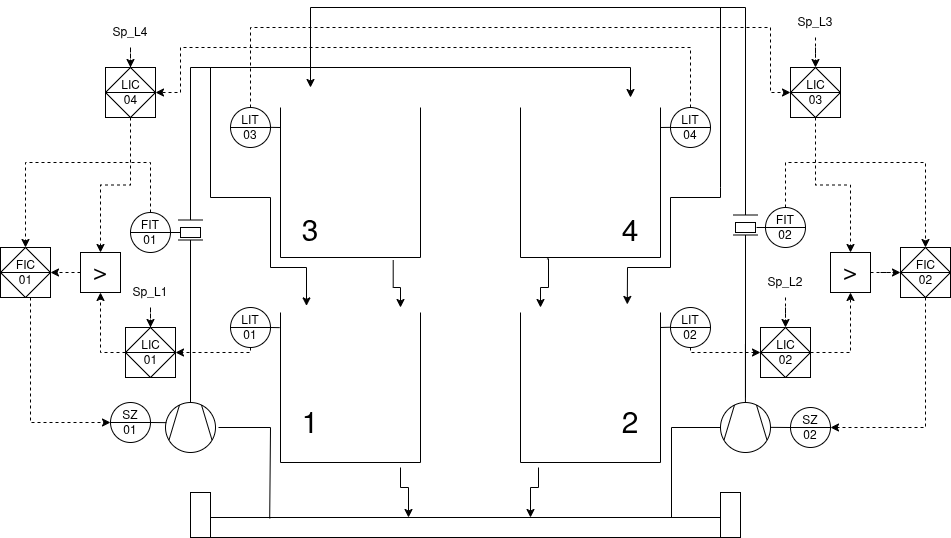
\includegraphics[width=0.95\textwidth]{figures/planta_4_estanques_P&ID.png}
  \end{center}
  \caption{P\&ID}\label{fig:pandi}
\end{figure}

\subsection{SAMA}

\begin{figure}[H]
  \begin{center}
    
\includegraphics[width=0.8\textwidth]{figures/sama.png}
  \end{center}
  \caption{sama}\label{fig:sama}
\end{figure}

\subsection{Bloques} 

\begin{figure}[H]
  \begin{center}
    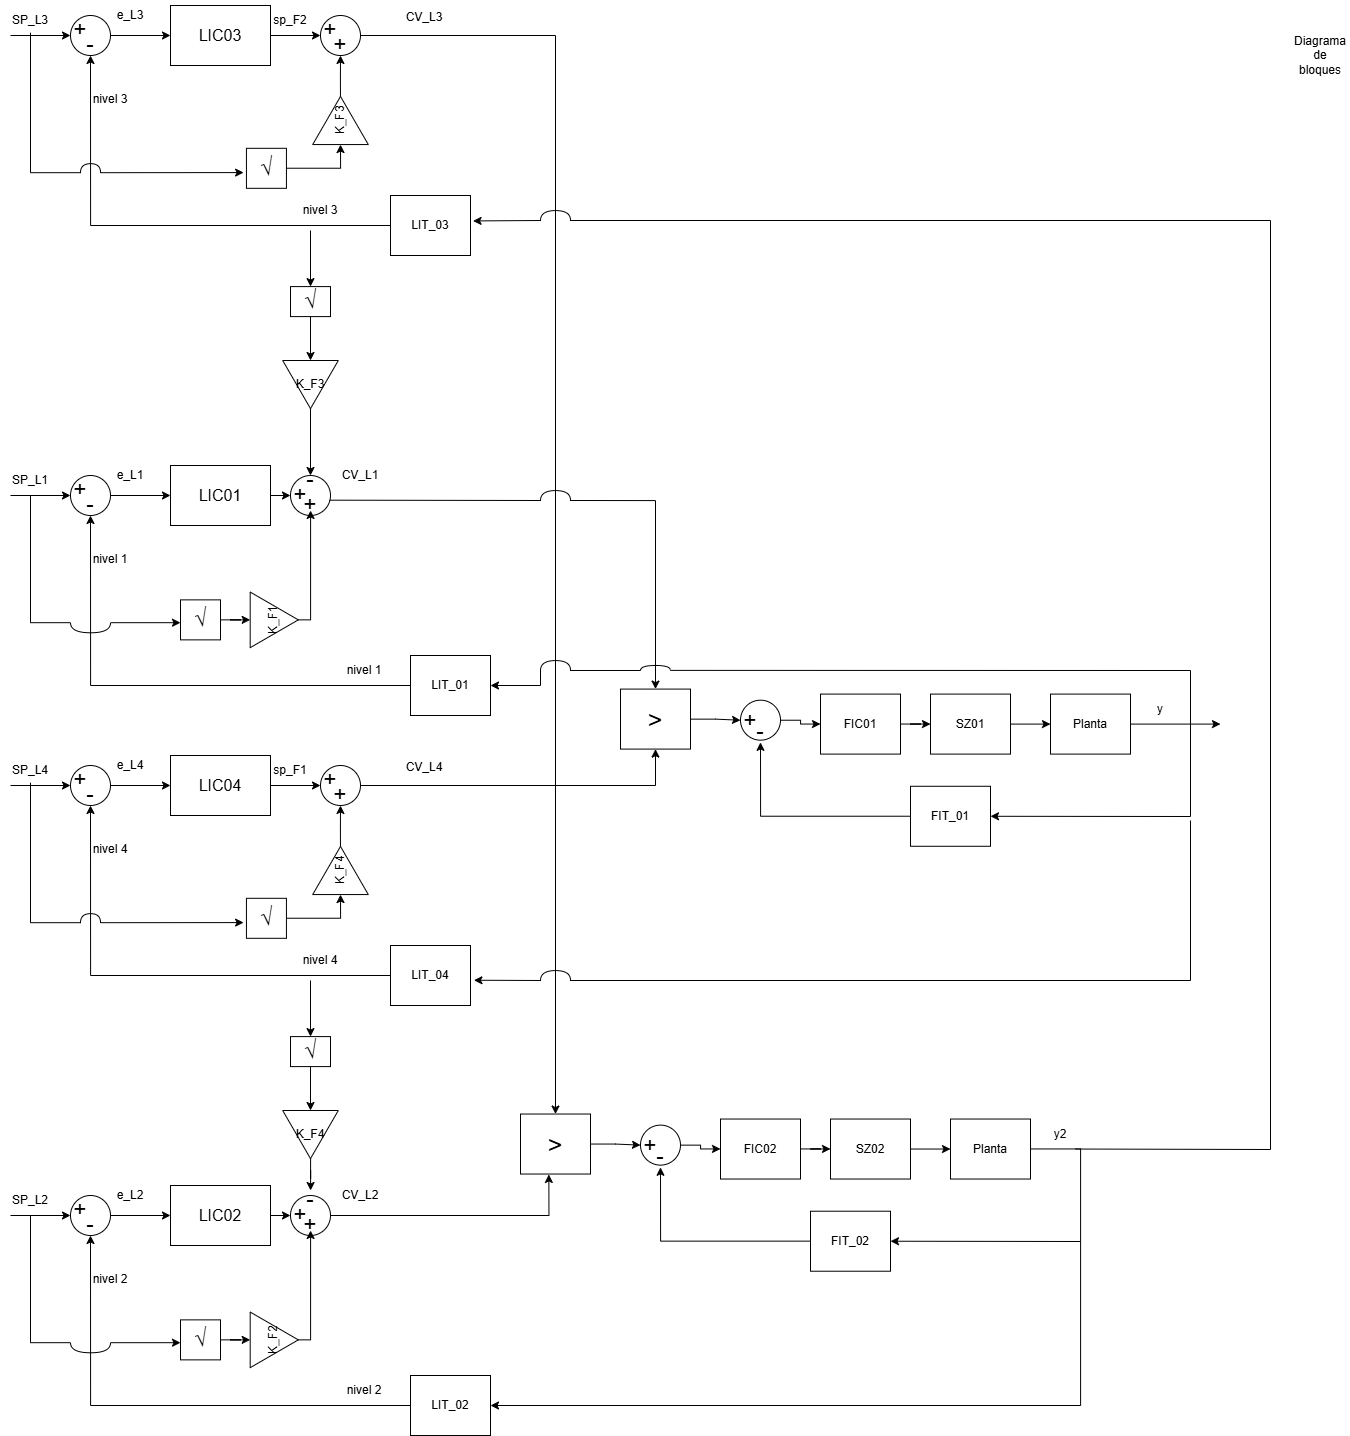
\includegraphics[width=0.8\textwidth]{figures/bloques_completo.png}
  \end{center}
  \caption{Bloques}\label{fig:bloques}
\end{figure}
\clearpage
\subsection{Norma ISA 101}
La norma ISA 101 detalla las características propias de una \textit{HUMAN-MACHINE-INTERFACE}, estas comprenden la ergonomía cognitiva y cuidado de la visión del operador. Características a destacar son:
\begin{itemize}
  \item Colores grises o claros
  \item Colores resaltantes (rojo, naranja, amarillos) solo para Alarmas o advertencias
  \item Jerarquía de pantallas, pantalla general, sintonización, alarmas, tendendencias, etc
  \item Alarmas, parada de planta y botones de navegación siempre disponibles
\end{itemize}

\begin{figure}[ht]
  \begin{center}
    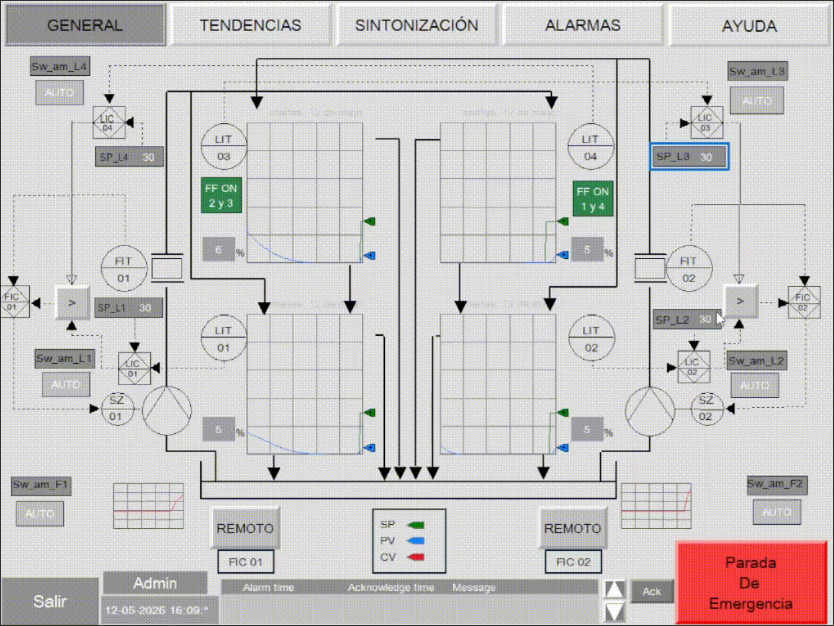
\includegraphics[width=0.8\textwidth]{figures/HMI.png}
  \end{center}
  \caption{HMI}\label{fig:HMI}
\end{figure}
\clearpage

